\documentclass[tikz,border=0pt]{standalone}
\usepackage{amsmath}
\usetikzlibrary{arrows.meta,positioning,calc}
\definecolor{bfill}{RGB}{232,240,250}\definecolor{bdraw}{RGB}{40,90,150}\definecolor{btxt}{RGB}{25,70,125}
\definecolor{ofill}{RGB}{252,238,224}\definecolor{odraw}{RGB}{190,95,20}\definecolor{otxt}{RGB}{160,75,10}
\definecolor{gfill}{RGB}{240,240,240}\definecolor{gdraw}{RGB}{110,110,110}
\newcommand{\ttl}{\fontsize{8}{9.5}\selectfont\bfseries}
\newcommand{\bdy}{\fontsize{7}{8.5}\selectfont}
\tikzset{
 box/.style={draw,rounded corners=2pt,line width=0.6pt,align=center,inner sep=2pt,font=\bdy},
 bbox/.style={box,fill=bfill,draw=bdraw},
 obox/.style={box,fill=ofill,draw=odraw},
 af/.style={-{Stealth[length=3.6pt,width=3.2pt]},line width=0.7pt},
 lab/.style={font=\bdy\itshape,inner sep=1pt},
}
\begin{document}
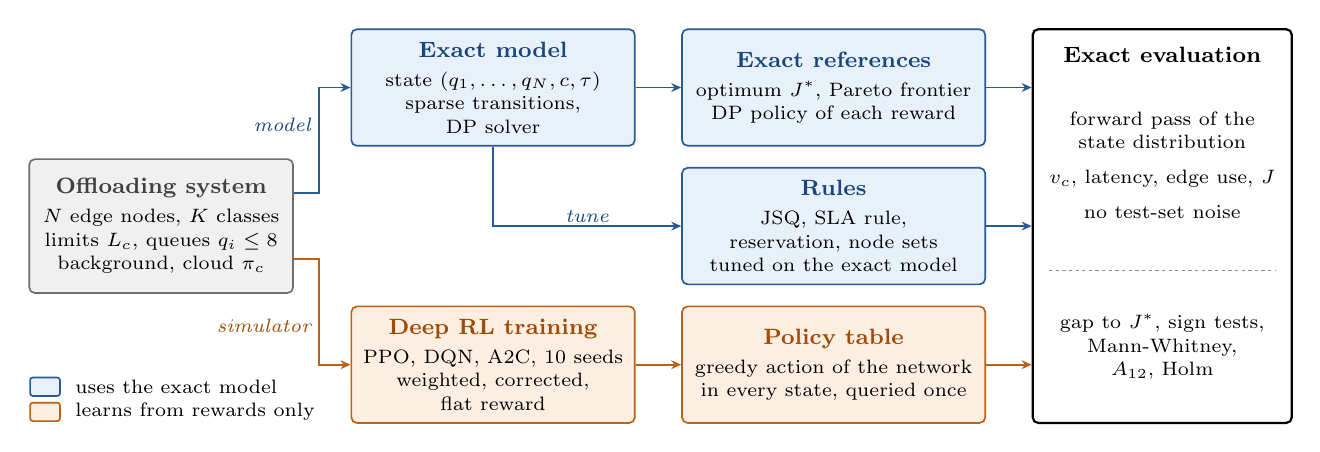
\begin{tikzpicture}
\def\W{16.06}\def\H{5.03}
\useasboundingbox (0,0) rectangle (\W,\H);
% columns
\def\xa{0.01}\def\wa{3.35}
\def\xb{4.10}\def\wb{3.60}
\def\xc{8.30}\def\wc{3.85}
\def\xd{12.75}
\def\ya{4.27}\def\yb{2.51}\def\yc{0.75}\def\hh{1.48}
% boxes
\node[box,fill=gfill,draw=gdraw,minimum width=\wa cm,minimum height=1.70cm,anchor=west] (sys) at (\xa,\yb)
 {{\ttl\color{black!75}Offloading system}\\[2pt]$N$ edge nodes, $K$ classes\\limits $L_c$, queues $q_i\le 8$\\background, cloud $\pi_c$};
\node[bbox,minimum width=\wb cm,minimum height=\hh cm,anchor=west] (mod) at (\xb,\ya)
 {{\ttl\color{btxt}Exact model}\\[2pt]state $(q_1,\dots,q_N,c,\tau)$\\sparse transitions,\\DP solver};
\node[obox,minimum width=\wb cm,minimum height=\hh cm,anchor=west] (rl) at (\xb,\yc)
 {{\ttl\color{otxt}Deep RL training}\\[2pt]PPO, DQN, A2C, 10 seeds\\weighted, corrected,\\flat reward};
\node[bbox,minimum width=\wc cm,minimum height=\hh cm,anchor=west] (ref) at (\xc,\ya)
 {{\ttl\color{btxt}Exact references}\\[2pt]optimum $J^*$, Pareto frontier\\DP policy of each reward};
\node[bbox,minimum width=\wc cm,minimum height=\hh cm,anchor=west] (rul) at (\xc,\yb)
 {{\ttl\color{btxt}Rules}\\[2pt]JSQ, SLA rule,\\reservation, node sets\\tuned on the exact model};
\node[obox,minimum width=\wc cm,minimum height=\hh cm,anchor=west] (tab) at (\xc,\yc)
 {{\ttl\color{otxt}Policy table}\\[2pt]greedy action of the network\\in every state, queried once};
\pgfmathsetmacro{\evw}{\W-\xd-0.02}
\pgfmathsetmacro{\evh}{\ya-\yc+\hh}
\node[box,fill=white,draw=black,line width=0.8pt,minimum width=\evw cm,minimum height=\evh cm,anchor=west] (ev) at (\xd,\yb) {};
\node[font=\ttl,anchor=north] (evt) at ($(ev.north)+(0,-0.12)$) {Exact evaluation};
\def\sepy{1.95}
\node[font=\bdy,align=center] at (ev.center|-0,{(\sepy+4.62)/2}) {forward pass of the\\state distribution\\[4pt]$v_c$, latency, edge use, $J$\\[4pt]no test-set noise};
\draw[black!45,line width=0.4pt,dash pattern=on 1.2pt off 1.2pt] ($(ev.west|-0,\sepy)+(0.22,0)$) -- ($(ev.east|-0,\sepy)+(-0.22,0)$);
\node[font=\bdy,align=center] at (ev.center|-0,{(\sepy+0.01)/2}) {gap to $J^*$, sign tests,\\Mann-Whitney,\\$A_{12}$, Holm};
% trunk from the system box
\def\tx{3.70}
\draw[af,bdraw] ($(sys.east)+(0,0.42)$) -| (\tx,\ya) -- (mod.west);
\draw[af,odraw] ($(sys.east)+(0,-0.42)$) -| (\tx,\yc) -- (rl.west);
\node[lab,text=btxt,anchor=east] at (\tx-0.06,3.80) {model};
\node[lab,text=otxt,anchor=east] at (\tx-0.06,1.25) {simulator};
% second column to third
\draw[af,bdraw] (mod.east) -- (ref.west);
\draw[af,bdraw] (mod.south) |- (rul.west) node[lab,text=btxt,pos=0.75,above] {tune};
\draw[af,odraw] (rl.east) -- (tab.west);
% into the evaluation
\draw[af,bdraw] (ref.east) -- (ref.east-|ev.west);
\draw[af,bdraw] (rul.east) -- (rul.east-|ev.west);
\draw[af,odraw] (tab.east) -- (tab.east-|ev.west);
% legend
\node[rounded corners=1pt,draw=bdraw,fill=bfill,line width=0.6pt,minimum width=0.38cm,minimum height=0.2cm,anchor=west] (l1) at (0.02,0.47) {};
\node[font=\bdy,anchor=west] at ($(l1.east)+(0.06,0)$) {uses the exact model};
\node[rounded corners=1pt,draw=odraw,fill=ofill,line width=0.6pt,minimum width=0.38cm,minimum height=0.2cm,anchor=west] (l2) at (0.02,0.15) {};
\node[font=\bdy,anchor=west] at ($(l2.east)+(0.06,0)$) {learns from rewards only};
\end{tikzpicture}
\end{document}
